\section{(6 points)}\label{ex:secu}

La loi de financement de la Sécurité sociale comprend un objectif national de dépenses d'assurance maladie, qui est voté chaque année par le Parlement.

Le montant des dépenses d'assurance maladie a été évalué pour l'année 2016 à \num{185.2} milliards d'euros. Le parlement a voté une croissance de ces dépenses de \num{2.1} \% pour l'année 2017.



\begin{questions}
	\question Montrer que le montant des dépenses  d'assurance maladie voté pour l'année 2017 est de \num{189.1} milliards d'euros \emph{(à cent millions près)}.
	
	\begin{solution}
		Le coefficient multiplicateur correspondant à une augmentation de \num{2.1} \%, est \num{1.021}.
		
		\begin{equation*}
			\num{185.2} \times \num{1.021} \approx \num{189.08}
		\end{equation*}
		
		Le montant des dépenses  d'assurance maladie voté pour l'année 2017 est donc bien de \num{189.1} milliards d'euros.
	\end{solution}
	
	
	
\end{questions}



Pour estimer les montants des années suivantes, on suppose que le Parlement votera chaque année une augmentation de \num{2.1} \% de ces dépenses.

On modélise à l'aide d'une suite $(v_n)$ le montant, en milliards d'euros des dépenses d'assurance maladie voté chaque année. On note $v_0$ le montant voté pour l'année 2016 et $v_n$ le montant voté pour l'année (2016 + $n$), où $n$ est un entier positif ou nul. On a ainsi $v_0 = \num{185.2}$.


 On veut utiliser la feuille de calcul automatisé ci-dessous afin d'obtenir les valeurs successives de la suite $(v_n)$.
 
 \begin{center}
 	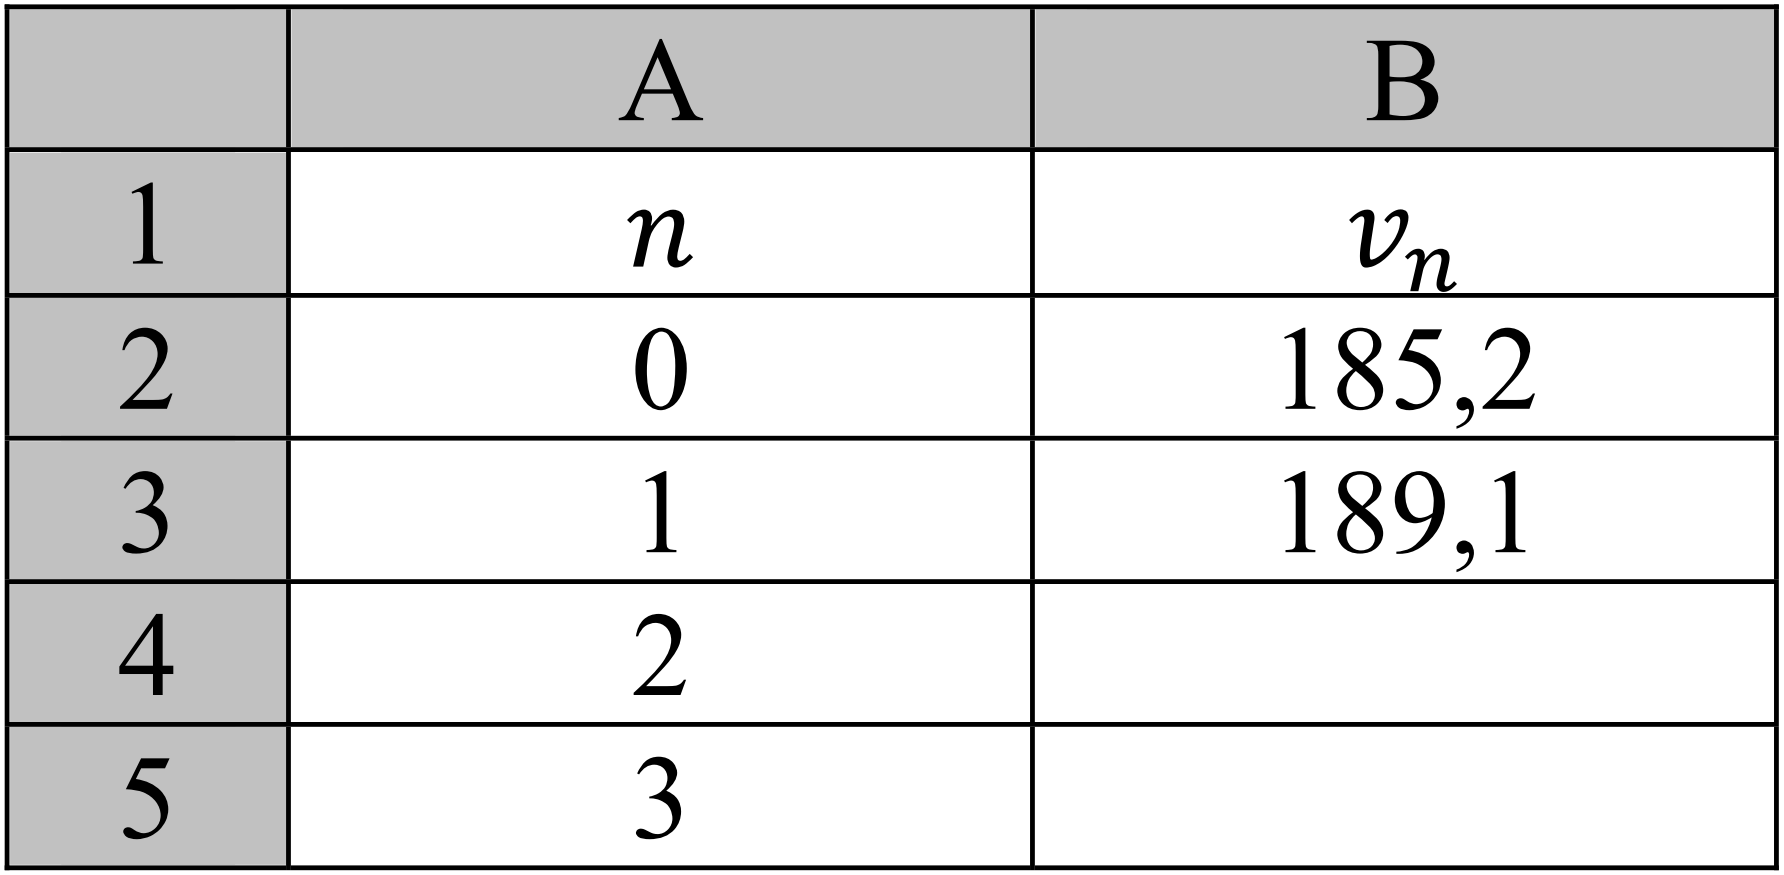
\includegraphics[scale=0.2]{img/secu}
 \end{center}

\begin{questions}
	\setcounter{question}{1}
	\question Quelle formule peut-on entrer dans la cellule $B3$, de sorte que, recopiée vers le bas, elle permette d'afficher les valeurs de la suite $(v_n)$ ?
	
	\begin{solution}
		Pour calculer les valeurs de la suite $(v_n)$, on rentre en $B4$ la formule suivante : 
		
		\begin{equation*}
			= B3 * \num{1.021}
		\end{equation*}
	\end{solution}

	\question Indiquer sans justification la nature de la suite $(v_n)$. Donner sa raison.
	
	\begin{solution}
		$(v_n)$ est une suite géométrique de raison \num{1.021}.
	\end{solution}
	
	\question Exprimer $v_n$ en fonction de $n$.
	\begin{solution}
		On a : 
		
		\begin{eqnarray*}
			v_n &=& v_0 \times q^n \\
			v_n &=& \num{185.2} \times \num{1.021}^n \\
		\end{eqnarray*}
	\end{solution}
	
	\question Déterminer une estimation de montant des dépenses d'assurance maladie voté par le parlement l'année 2020. \emph{(Arrondir la valeur à la centaine de millions.)}
	\begin{solution}
		L'année 2020 est l'année de rang 4 (2016 + 4), je calcule $v_4$ :
		
		\begin{eqnarray*}
			v_4 &=& \num{185.2} \times \num{1.021}^4 \\
			v_4 & \approx & \num{201.4}
		\end{eqnarray*}
		
		Avec ce modèle, on peut estimer le montant des dépenses d'assurance maladie voté par le parlement l'année 2020 à \num{201.4} milliards d'euros.
	\end{solution}
	
	\question \`A l'aide de la calculatrice, trouver la valeur de $x$ telle que $\num{185.2} \times \num{1.021}^x \ge \num{210}$.
	
	\begin{solution}
		\`A l'aide de la calculatrice j'obtiens $v_6 \approx \num{2019.8}$ et $v_7 \approx \num{214.2}$. On a donc $\num{185.2} \times \num{1.021}^x \ge \num{210}$ pour $x \ge 7$. 
	\end{solution}
	
	\question Déterminer, suivant ce modèle, l'année pour laquelle sera voté, pour la première fois, un montant de dépenses de l'assurance maladie supérieur à 210 milliards d'euros. 
	
	\begin{solution}
		Selon ce modèle, un montant de dépenses de l'assurance maladie supérieur à 210 milliards d'euros, sera voté pour la première fois en 2023 (2016 + 7).
	\end{solution}
\end{questions}